\documentclass[tikz,border=10pt]{standalone}
\usepackage{amsmath}
\usepackage{tikz}
\usetikzlibrary{arrows.meta, positioning, calc, shapes.geometric}

\begin{document}
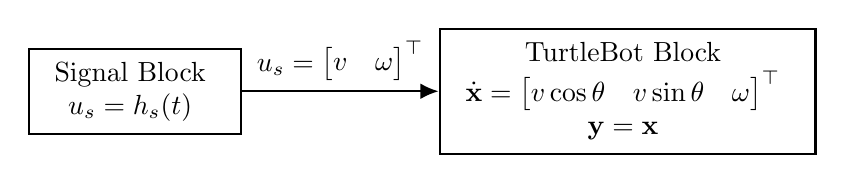
\begin{tikzpicture}[
  block/.style = {draw, thick, minimum height=3em, minimum width=6em, align=center},
  circ/.style  = {draw, circle, thick, minimum size=2.5em, inner sep=0pt},
  gain/.style  = {draw, isosceles triangle, isosceles triangle apex angle=60,
                  shape border rotate=135, % apex points LEFT
                  minimum height=2em, minimum width=2em, thick, inner sep=0pt},
  arrow/.style = {thick, -{Latex[width=2mm]}},
  node distance=2.5cm and 2.5cm
]

  % Signal Generator
  \node[block] (siggen) {
    \begin{tabular}{c}
      Signal Block \\
      $u_s = h_s(t)$
    \end{tabular}
  };

  % Plant (right of siggen)
  \node[block, right=2.5cm of siggen] (system) {
    \begin{tabular}{c}
      TurtleBot Block \\
      $\displaystyle
      \dot{\mathbf{x}} =
      \begin{bmatrix}
        v \cos\theta &
        v \sin\theta &
        \omega
      \end{bmatrix}^{\top}$ \\
      $\mathbf{y} = \mathbf{x}$
    \end{tabular}
  };

  % Connection
  \draw[arrow] (siggen.east) -- node[above] {$u_s=\begin{bmatrix} v & \omega \end{bmatrix}^{\top}$} (system.west);

\end{tikzpicture}
\end{document}
